%%%%%%%%%%%%%%%%%%%%%%%%%%%%%%%%%%%%%%%%%
% Beamer Presentation
% LaTeX Template
% Version 1.0 (10/11/12)
%
% This template has been downloaded from:
% http://www.LaTeXTemplates.com
%
% License:
% CC BY-NC-SA 3.0 (http://creativecommons.org/licenses/by-nc-sa/3.0/)
%
%%%%%%%%%%%%%%%%%%%%%%%%%%%%%%%%%%%%%%%%%

%----------------------------------------------------------------------------------------
%	PACKAGES AND THEMES
%----------------------------------------------------------------------------------------

\documentclass[handout]{beamer}

\mode<presentation> {

% The Beamer class comes with a number of default slide themes
% which change the colors and layouts of slides. Below this is a list
% of all the themes, uncomment each in turn to see what they look like.

%\usetheme{default}
%\usetheme{AnnArbor}
%\usetheme{Antibes}
%\usetheme{Bergen}
%\usetheme{Berkeley}
%\usetheme{Berlin}
%\usetheme{Boadilla}
%\usetheme{CambridgeUS}
%\usetheme{Copenhagen}
%\usetheme{Darmstadt}
%\usetheme{Dresden}
%\usetheme{Frankfurt}
%\usetheme{Goettingen}
%\usetheme{Hannover}
%\usetheme{Ilmenau}
%\usetheme{JuanLesPins}
%\usetheme{Luebeck}
\usetheme{Madrid}
%\usetheme{Malmoe}
%\usetheme{Marburg}
%\usetheme{Montpellier}
%\usetheme{PaloAlto}
%\usetheme{Pittsburgh}
%\usetheme{Rochester}
%\usetheme{Singapore}
%\usetheme{Szeged}
%\usetheme{Warsaw}

% As well as themes, the Beamer class has a number of color themes
% for any slide theme. Uncomment each of these in turn to see how it
% changes the colors of your current slide theme.

%\usecolortheme{albatross}
%\usecolortheme{beaver}
%\usecolortheme{beetle}
%\usecolortheme{crane}
%\usecolortheme{dolphin}
%\usecolortheme{dove}
%\usecolortheme{fly}
%\usecolortheme{lily}
%\usecolortheme{orchid}
%\usecolortheme{rose}
%\usecolortheme{seagull}
%\usecolortheme{seahorse}
%\usecolortheme{whale}
%\usecolortheme{wolverine}

%\setbeamertemplate{footline} % To remove the footer line in all slides uncomment this line
%\setbeamertemplate{footline}[page number] % To replace the footer line in all slides with a simple slide count uncomment this line

%\setbeamertemplate{navigation symbols}{} % To remove the navigation symbols from the bottom of all slides uncomment this line
}

\usepackage{graphicx} % Allows including images
\usepackage{booktabs} % Allows the use of \toprule, \midrule and \bottomrule in tables
\usepackage{cool}
\usepackage{amsmath}
\usepackage{amssymb}
\usepackage{bm}
\usepackage{physics}
\usepackage{hyperref}
\usepackage{listings}

\DeclareMathOperator*{\argmax}{argmax}
\DeclareMathOperator*{\argmin}{argmin}

%----------------------------------------------------------------------------------------
%	TITLE PAGE
%----------------------------------------------------------------------------------------

\title[Markov Process Chapter]{A Guided Tour of \href{http://stanford.edu/~ashlearn/RLForFinanceBook/book.pdf}{\underline{\textcolor{yellow}{Chapter 1}}}: \\  Markov Process and Markov Reward Process} % The short title appears at the bottom of every slide, the full title is only on the title page

\author{Ashwin Rao} % Your name
\institute[Stanford] % Your institution as it will appear on the bottom of every slide, may be shorthand to save space
{ICME, Stanford University
 % Your institution for the title page
}

\date % Date, can be changed to a custom date

\begin{document}
\lstset{language=Python}  
\begin{frame}
\titlepage % Print the title page as the first slide
\end{frame}

% \begin{frame}
% \frametitle{Overview} % Table of contents slide, comment this block out to remove it
% \tableofcontents % Throughout your presentation, if you choose to use \section{} and \subsection{} commands, these will automatically be printed on this slide as an overview of your presentation
% \end{frame}

\begin{frame}
\frametitle{Intuition on the concepts of {\em Process} and {\em State}}
\pause
\begin{itemize}[<+->]
\item {\em Process:} time-sequenced random outcomes
\item Random outcome eg: price of a derivative, portfolio value etc.
\item {\em State:} Internal Representation $S_t$ driving future evolution
\item We are interested in $\mathbb{P}[S_{t+1}|S_t, S_{t-1}, \ldots, S_0]$
\item Let us consider random walks of stock prices $X_t = S_t$
$$\mathbb{P}[X_{t+1} = X_t + 1] + \mathbb{P}[X_{t+1} = X_t - 1] = 1$$
\item We consider 3 examples of such processes
\end{itemize}
\end{frame}

\begin{frame}
\frametitle{Markov Property - Stock Price Random Walk Process}
\pause
\begin{itemize}[<+->]
\item Process is pulled towards level $L$ with strength parameter $\alpha$
$$\mathbb{P}[X_{t+1} = X_t + 1] = \frac 1 {1 + e^{-\alpha_1(L - X_t)}}$$
\item Notice how the probability of next price depends only on current price
\item ``The future is independent of the past given the present''
$$\mathbb{P}[X_{t+1}|X_t, X_{t-1}, \ldots, X_0] = \mathbb{P}[X_{t+1}|X_t]\text{ for all } t \geq 0$$
\item This makes the mathematics easier and the computation tractable
\item We call this the {\em Markov Property} of States
\item The state captures all relevant information from history
\item Once the state is known, the history may be thrown away
\item The state is a sufficient statistic of the future
\end{itemize}
\end{frame}

\begin{frame}
\frametitle{Logistic Functions $f(x;\alpha) = \frac 1 {1 + e^{-\alpha x}}$}
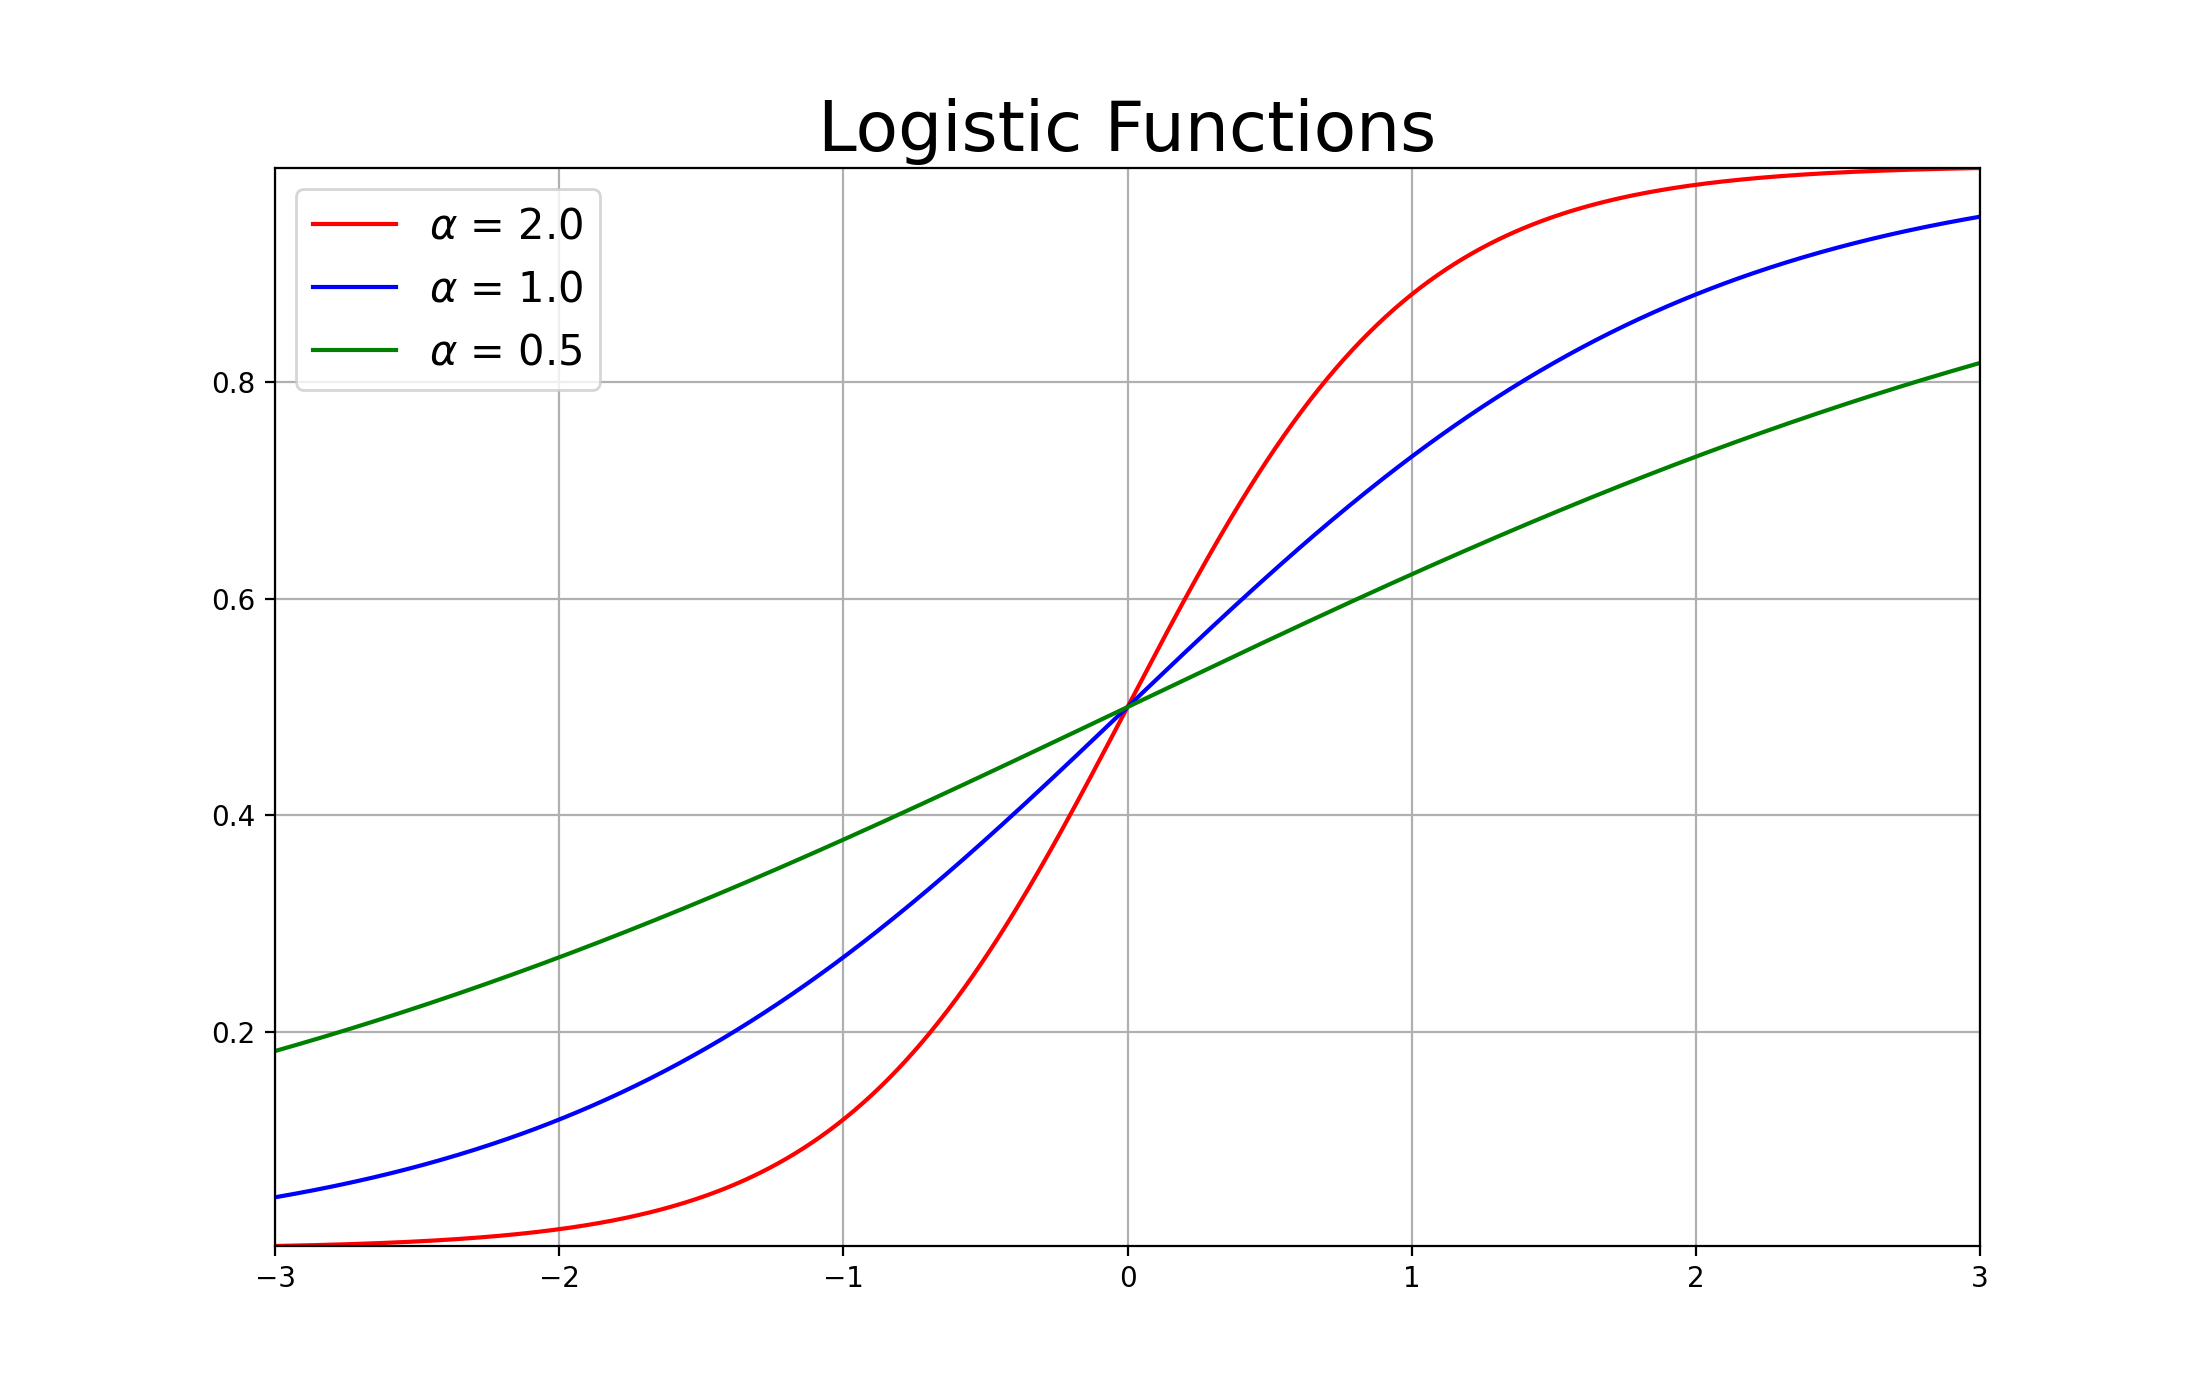
\includegraphics[width=12cm, height=7cm]{logistic_curves.png}
\end{frame}

\begin{frame}
\frametitle{Another Stock Price Random Walk Process}
\pause
$$
\mathbb{P}[X_{t+1} = X_t + 1] =
\begin{cases}
0.5 (1 - \alpha_2(X_t - X_{t-1})) & \text{if } t > 0\\
0.5 & \text{if } t = 0
\end{cases}
$$
\begin{itemize}[<+->]
\item Direction of $X_{t+1} - X_t$ is biased in the reverse direction of $X_t - X_{t-1}$
\item Extent of the bias is controlled by ``pull-strength'' parameter $\alpha_2$
\item $S_t  = X_t$ doesn't satisfy Markov Property, $S_t = (X_t, X_t - X_{t-1})$ does
$$\mathbb{P}[(X_{t+1}, X_{t+1} - X_t)|(X_t, X_t - X_{t-1}), (X_{t-1}, X_{t-1} - X_{t-2}), \ldots, (X_0, Null)]$$
$$= \mathbb{P}[(X_{t+1}, X_{t+1} - X_t)|(X_t, X_t - X_{t-1})] $$
\item $S_t = (X_0, X_1, \ldots, X_t)$ or $S_t = (X_t, X_{t-1})$ also satisfy Markov Property
\item But we seek the  "simplest/minimal" representation for Markov State
\end{itemize}
\end{frame}

\begin{frame}
\frametitle{Yet Another Stock Price Random Walk Process}
\pause
\begin{itemize}[<+->]
\item Here, probability of next move depends on {\em all} past moves
\item Depends on \# past up-moves $U_t$ relative to \# past down-moves $D_t$
$$
\mathbb{P}[X_{t+1} = X_t + 1] =
\begin{cases}
\frac 1 {1 + (\frac {U_t + D_t} {D_t} - 1)^{\alpha_3}} & \text{if } t > 0\\
0.5 & \text{if } t = 0
\end{cases}
$$
\item Direction of $X_{t+1} - X_t$ biased in the reverse direction of history
\item $\alpha_3$ is a ``pull-strength'' parameter
\item Most ``compact'' Markov State $S_t = (U_t, D_t)$
$$\mathbb{P}[(U_{t+1}, D_{t+1})|(U_t, D_t), (U_{t-1}, D_{t-1}), \ldots, (U_0, D_0)]$$
$$ = \mathbb{P}[(U_{t+1}, D_{t+1})|(U_t, D_t)]$$
\item Note that $X_t$ is not part of $S_t$ since $X_t = X_0 + U_t - D_t$
\end{itemize}
\end{frame}

\begin{frame}
\frametitle{Unit-Sigmoid Curves $f(x; \alpha) = \frac 1 {1 + (\frac 1 x - 1)^{\alpha}}$}
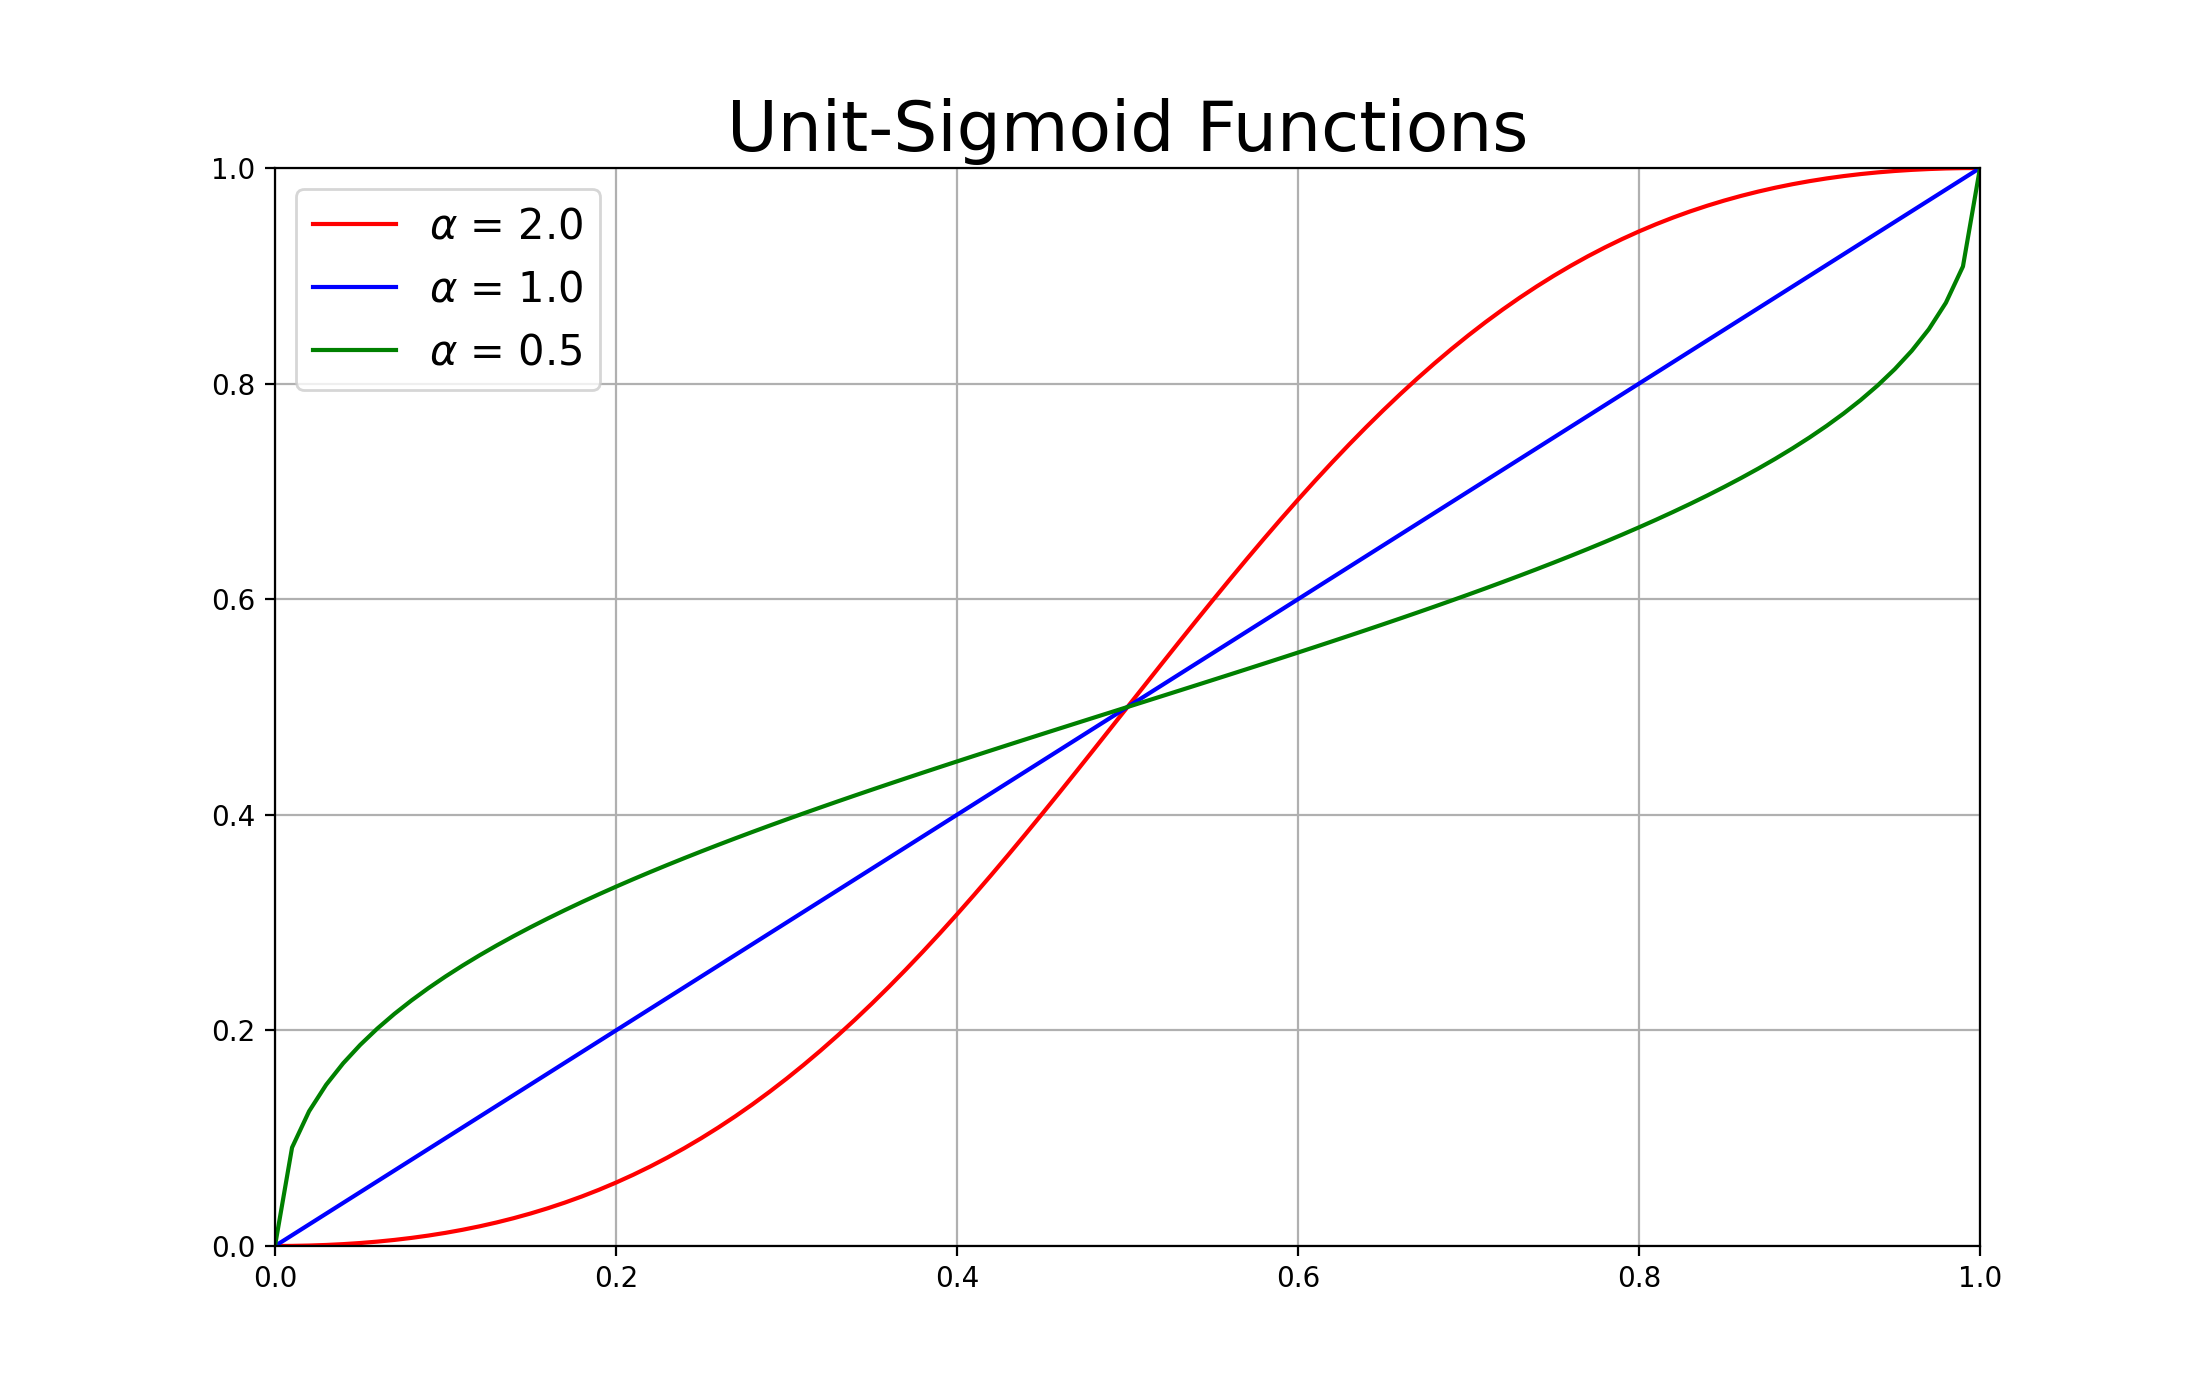
\includegraphics[width=12cm, height=7cm]{unit_sigmoid_curves.png}
\end{frame}

\begin{frame}
\frametitle{Single Sampling Traces for the 3 Processes}
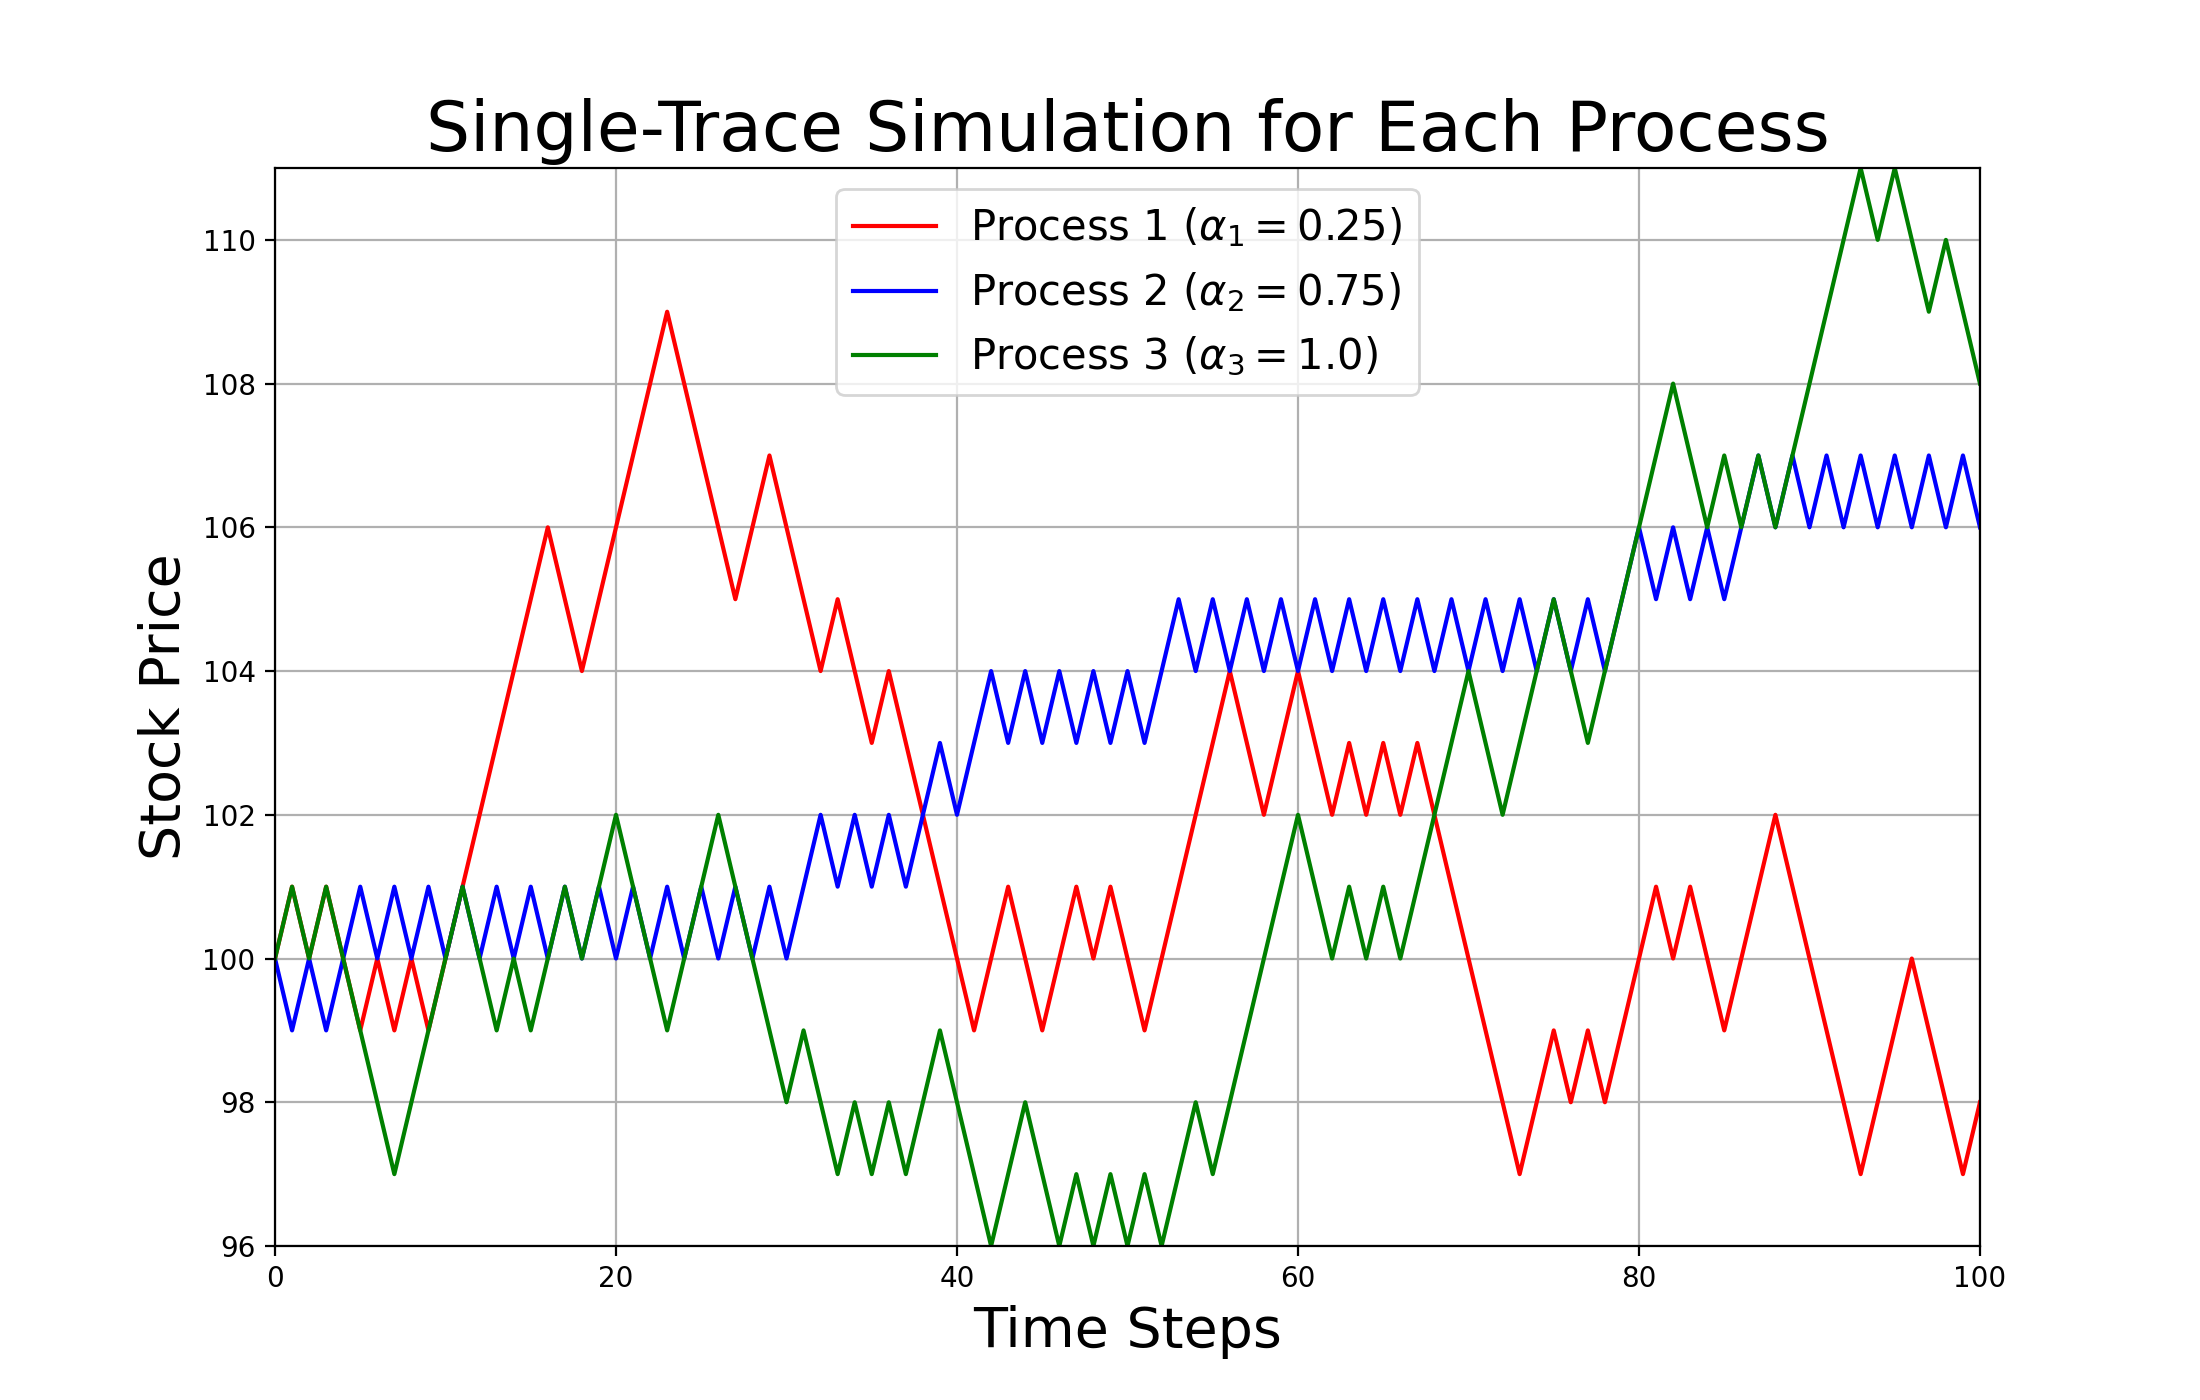
\includegraphics[width=12cm, height=7cm]{single_traces.png}
\end{frame}

\begin{frame}
\frametitle{Terminal Probability Distributions for the 3 Processes}
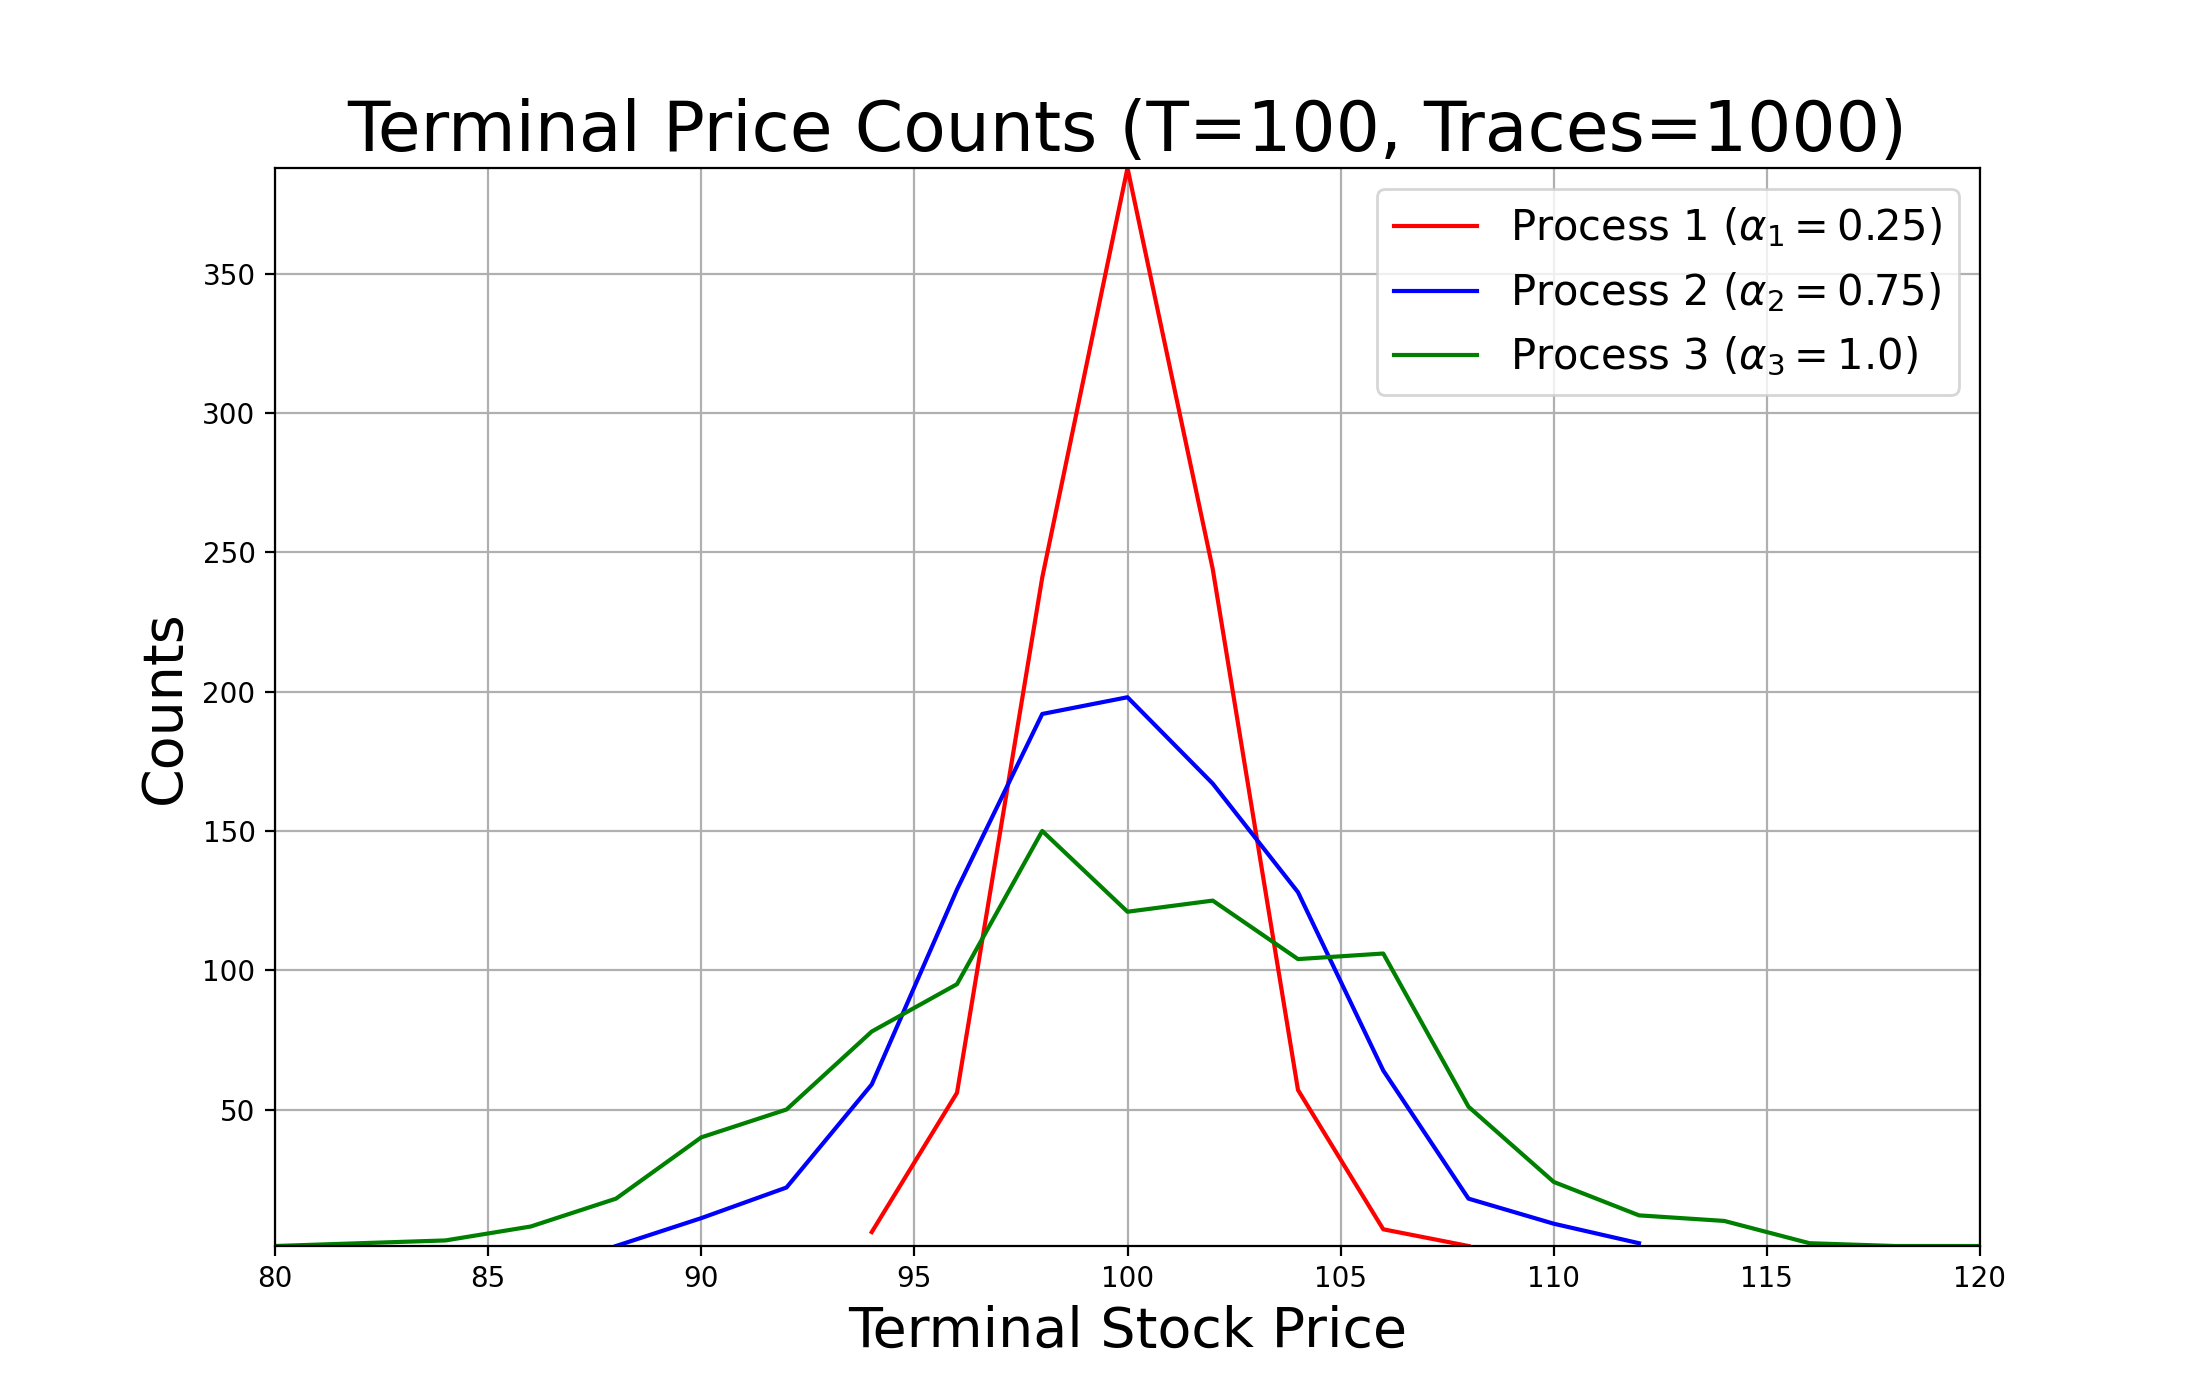
\includegraphics[width=12cm, height=7cm]{terminal_distribution.png}
\end{frame}

\begin{frame}
\frametitle{Definition for Discrete Time, Countable States}
\pause
\begin{definition}
A {\em Markov Process} consists of:
\begin{itemize}
\item A countable set of states $\mathcal{S}$ (known as the State Space) and a set $\mathcal{T} \subseteq \mathcal{S}$ (known as the set of Terminal States)
\item A time-indexed sequence of random states $S_t \in \mathcal{S}$ for time steps $t=0, 1, 2, \ldots$ with each state transition satisfying the Markov Property: $\mathbb{P}[S_{t+1}|S_t, S_{t-1}, \ldots, S_0] = \mathbb{P}[S_{t+1}|S_t]$ for all $t \geq 0$
\item Termination: If an outcome for $S_T$ (for some time step $T$) is a state in the set $\mathcal{T}$, then this sequence outcome terminates at time step $T$
\end{itemize}
\end{definition}
\pause
\begin{itemize}[<+->]
\item The more commonly used term for {\em Markov Process} is {\em Markov Chain}
\item We refer to $\mathbb{P}[S_{t+1}|S_t]$ as the transition probabilities for time $t$.
\item Non-terminal states: $\mathcal{N} = \mathcal{S} - \mathcal{T}$
\item Classical Finance results based on continuous-time Markov Processes
\end{itemize}
\end{frame}

\begin{frame}
\frametitle{Some nuances of Markov Processes}
\pause
\begin{itemize}[<+->]
\item Stationary Markov Process: $\mathbb{P}[S_{t+1}|S_t]$ independent of $t$
\item Stationary Markov Process specified with function $\mathcal{P}: \mathcal{N} \times \mathcal{S} \rightarrow [0,1]$
$$\mathcal{P}(s, s') = \mathbb{P}[S_{t+1}=s'|S_t=s] \text{ for all } t = 0, 1, 2, \ldots$$
\item $\mathcal{P}$ is the {\em Transition Probability Function} (source $s \rightarrow$ destination $s'$)
\item Convert non-Stationary to Stationary by augmenting {\em State} with time
\item Default: {\em Discrete-Time, Countable-States Stationary Markov Process}
\item Termination typically modeled with {\em Absorbing States} (we don't!)
\item Separation between:
\begin{itemize}
\item Specification of Transition Probability Function $\mathcal{P}$
\item Specification of Probability Distribution of Start States $\mu: \mathcal{S} \rightarrow [0, 1]$ 
\end{itemize}
\item Together ($\mathcal{P}$ and $\mu$), we can produce {\em Sampling Traces}
\item {\em Episodic} versus {\em Continuing} Sampling Traces
\end{itemize}
\end{frame}

\begin{frame}[fragile]
\frametitle{The @abstractclass MarkovProcess}
\pause
\begin{lstlisting}
class MarkovProcess(ABC, Generic[S]):

    @abstractmethod
    def transition(self, state: NonTerminal[S]) -> \
            Distribution[State[S]]:
        pass

    def simulate(
        self,
        start_st_distr: Distribution[NonTerminal[S]]
    ) -> Iterable[State[S]]:
        st: State[S] = start_state_distr.sample()
        yield st
        while isinstance(st, NonTerminal):
            st = self.transition(st).sample()
            yield st
\end{lstlisting}
\end{frame}

\begin{frame}[fragile]
\frametitle{Finite Markov Process}
\pause
\begin{itemize}[<+->]
\item Finite State Space $\mathcal{S} = \{s_1, s_2, \ldots, s_n\}$, $|\mathcal{N}| = m\leq n$
\item We'd like a {\em sparse representation} for $\mathcal{P}$
\item Conceptualize $\mathcal{P} : \mathcal{N} \times \mathcal{S} \rightarrow [0, 1]$ as $\mathcal{N} \rightarrow (\mathcal{S} \rightarrow [0, 1])$
\end{itemize}
\pause
\begin{lstlisting}
Transition = Mapping[
    NonTerminal[S],
    FiniteDistribution[State[S]]
]
\end{lstlisting}
\end{frame}


\begin{frame}[fragile]
\frametitle{class FiniteMarkovProcess}
\pause
\begin{lstlisting}
class FiniteMarkovProcess(MarkovProcess[S]):

    nt_states: Sequence[NonTerminal[S]]
    tr_map: Transition[S]

    def __init__(self, tr: Mapping[S,
            FiniteDistribution[S]]):
        nt: Set[S] = set(tr.keys())
        self.tr_map = {
            NonTerminal(s): Categorical(
                {(NonTerminal(s1) if s1 in nt else
                 Terminal(s1)): p
                 for s1, p in v.table().items()}
            ) for s, v in tr.items()
        }
        self.nt_states = list(self.tr_map.keys())
        
    def transition(self, state: NonTerminal[S])\
        -> FiniteDistribution[State[S]]:
    return self.tr_map[state]
\end{lstlisting}
\end{frame}

\begin{frame}[fragile]
\frametitle{class FiniteMarkovProcess}
\pause
\begin{lstlisting}        
    def transition(self, state: NonTerminal[S])\
        -> FiniteDistribution[State[S]]:
    return self.tr_map[state]
\end{lstlisting}
\end{frame}


\begin{frame}[fragile]
\frametitle{Weather Finite Markov Process}
\begin{lstlisting}       
{
  "Rain": Categorical({"Rain": 0.3, "Nice": 0.7}),
  "Snow": Categorical({"Rain": 0.4, "Snow": 0.6}),
  "Nice": Categorical({
      "Rain": 0.2,
      "Snow": 0.3,
      "Nice": 0.5
  })
}
\end{lstlisting}
\end{frame}

\begin{frame}
\frametitle{Weather Finite Markov Process}
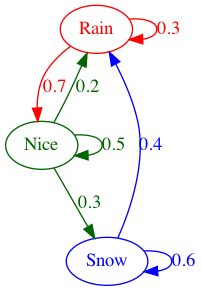
\includegraphics[width=10cm, height=8cm]{weather_mp.png}
\end{frame}


\begin{frame}
\frametitle{Order of Activity for Inventory Markov Process}
\pause
$\alpha$ := On-Hand Inventory, $\beta$ := On-Order Inventory, $C$ := Store Capacity
\pause
\begin{itemize}[<+->]
\item Observe State $S_t$: $(\alpha, \beta)$ at 6pm store-closing
\item Order Quantity := $\max(C - (\alpha + \beta), 0)$
\item Receive Inventory at 6am if you had ordered 36 hrs ago
\item Open the store at 8am
\item Experience random demand $i$ with poisson probabilities:
$$\text{PMF } f(i) = \frac {e^{-\lambda} \lambda^i} {i!}, \text{ CMF } F(i) = \sum_{j=0}^i f(j)$$
\item Inventory Sold is $\max(\alpha + \beta, i)$
\item Close the store at 6pm
\item Observe new state $S_{t+1}: (\max(\alpha + \beta - i, 0), \max(C - (\alpha + \beta), 0))$
\end{itemize}
\end{frame}

\begin{frame}
\frametitle{Inventory Markov Process States and Transitions}
\pause
$$\mathcal{S} := \{(\alpha, \beta) : 0 \leq \alpha + \beta \leq C\}$$
\pause
$$\text{If } S_t := (\alpha, \beta), S_{t+1} := (\alpha + \beta - i, C - (\alpha + \beta)) \text{ for } i =0, 1, \ldots, \alpha + \beta$$
\pause
$$\mathcal{P}((\alpha, \beta), (\alpha + \beta - i, C - (\alpha + \beta))) = f(i)\text{ for } 0 \leq i \leq \alpha + \beta - 1$$
\pause
$$\mathcal{P}((\alpha, \beta), (0, C - (\alpha + \beta))) = \sum_{j=\alpha+\beta}^{\infty} f(j) = 1 - F(\alpha + \beta - 1)$$
\end{frame}

\begin{frame}
\frametitle{Inventory Markov Process}
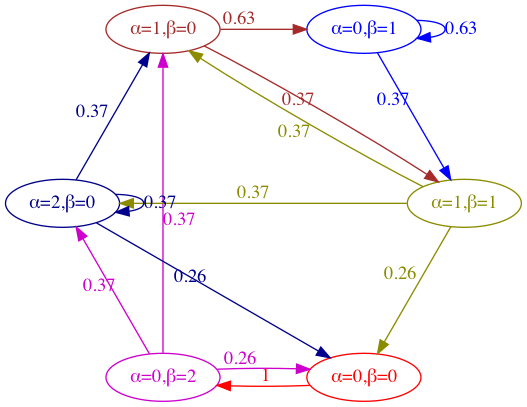
\includegraphics[width=12cm, height=8cm]{simple_inv_mp.png}
\end{frame}

\begin{frame}
\frametitle{Stationary Distribution of a Markov Process}
\pause
\begin{definition} 
 The {\em Stationary Distribution} of a (Stationary) Markov Process with state space $\mathcal{S} = \mathcal{N}$ and transition probability function $\mathcal{P}: \mathcal{N} \times \mathcal{N} \rightarrow [0, 1]$ is a probability distribution function $\pi: \mathcal{N} \rightarrow [0, 1]$ such that:
  $$\pi(s) = \sum_{s'\in \mathcal{N}} \pi(s) \cdot \mathcal{P}(s', s) \text{ for all } s \in \mathcal{N}$$
\end{definition}
\pause
For Stationary Process with finite states $\mathcal{S} = \{s_1, s_2, \ldots, s_n\} = \mathcal{N}$,
$$\pi(s_j) = \sum_{i=1}^n \pi(s_i) \cdot \mathcal{P}(s_i, s_j) \text{ for all } j = 1, 2, \ldots n$$
\pause
Turning $\mathcal{P}$ into a matrix, we get: $\bm{\pi}^T = \bm{\pi}^T \cdot \bm{\mathcal{P}}$\\
\pause
$\bm{\mathcal{P}}^T \cdot \bm{\pi}= \bm{\pi} \Rightarrow \bm{\pi}$ is an eigenvector of $\bm{\mathcal{P}}^T$ with eigenvalue of 1
\end{frame}


\begin{frame}
\frametitle{MRP Definition for Discrete Time, Countable States}
\pause
\begin{definition}
 A {\em Markov Reward Process (MRP)} is a Markov Process, along with a time-indexed sequence of {\em Reward} random variables $R_t \in \mathcal{D}$ (a countable subset of $\mathbb{R}$) for time steps $t=1, 2, \ldots$, satisfying the Markov Property (including Rewards): $\mathbb{P}[(R_{t+1}, S_{t+1}) | S_t, S_{t-1}, \ldots, S_0] = \mathbb{P}[(R_{t+1}, S_{t+1}) | S_t]$ for all $t \geq 0$.
 \end{definition}
 \pause
  $$S_0, R_1, S_1, R_2, S_2, \ldots, S_{T-1}, R_T, S_T$$
  \pause
 \begin{itemize}[<+->]
\item By default, assume stationary: $\mathbb{P}[(R_{t+1}, S_{t+1}) | S_t]$ independent of $t$
\item Stationary MRP specified with function $\mathcal{P}_R: \mathcal{N} \times \mathcal{D} \times \mathcal{S} \rightarrow [0,1]$
$$\mathcal{P}_R(s,r,s') = \mathbb{P}[(R_{t+1}=r, S_{t+1}=s') | S_t=s] \text{ for all } t = 0, 1, 2, \ldots$$
\item $\mathcal{P}_R$ known as the {\em Transition Probability Function}
\end{itemize}
\end{frame}


\begin{frame}[fragile]
\frametitle{@abstractclass MarkovRewardProcess}
\pause
\begin{lstlisting}
class MarkovRewardProcess(MarkovProcess[S]):

    @abstractmethod
    def transition_reward(self, state: NonTerminal[S])\
            -> Distribution[Tuple[State[S], float]]:
        pass
        
    def transition(self, state: NonTerminal[S]) \
            -> Distribution[State[S]]:
        distribution = self.transition_reward(state)

        def next_state(distribution=distribution):
            next_s, _ = distribution.sample()
            return next_s

        return SampledDistribution(next_state)
\end{lstlisting}            
\end{frame}

\begin{frame}
\frametitle{MRP Reward Functions}
\pause
\begin{itemize}[<+->]
\item The reward transition function $\mathcal{R}_T: \mathcal{N} \times \mathcal{S} \rightarrow \mathbb{R}$ is defined as:
$$\mathcal{R}_T(s,s') = \mathbb{E}[R_{t+1}|S_{t+1}=s',S_t=s]$$
$$ = \sum_{r\in \mathcal{D}} \frac {\mathcal{P}_R(s,r,s')} {\mathcal{P}(s,s')} \cdot r = \sum_{r\in \mathcal{D}} \frac {\mathcal{P}_R(s,r,s')} {\sum_{r\in \mathcal{D}} \mathcal{P}_R(s,r,s')} \cdot r$$
\item The reward function $\mathcal{R}: \mathcal{N} \rightarrow \mathbb{R}$ is defined as:
$$\mathcal{R}(s) = \mathbb{E}[R_{t+1}|S_t=s]$$
$$ = \sum_{s' \in \mathcal{S}} \mathcal{P}(s,s') \cdot \mathcal{R}_T(s,s') = \sum_{s'\in \mathcal{S}} \sum_{r \in \mathcal{D}} \mathcal{P}_R(s,r,s') \cdot r$$
\end{itemize}
\end{frame}

\begin{frame}
\frametitle{Inventory MRP}
\pause
\begin{itemize}[<+->]
\item Embellish Inventory Process with Holding Cost and Stockout Cost
\item Holding cost of $h$ for each unit that remains overnight
\item Think of this as ``interest on inventory'', also includes upkeep cost
\item Stockout cost of $p$ for each unit of ``missed demand''
\item For each customer demand you could not satisfy with store inventory
\item Think of this as lost revenue plus customer disappointment ($p \gg h$)
\end{itemize}
\end{frame}

\begin{frame}
\frametitle{Order of Activity for Inventory MRP}
\pause
$\alpha$ := On-Hand Inventory, $\beta$ := On-Order Inventory, $C$ := Store Capacity
\pause
\begin{itemize}[<+->]
\item Observe State $S_t$: $(\alpha, \beta)$ at 6pm store-closing
\item Order Quantity := $\max(C - (\alpha + \beta), 0)$
\item Record any overnight holding cost ($=h \cdot \alpha$)
\item Receive Inventory at 6am if you had ordered 36 hours ago
\item Open the store at 8am
\item Experience random demand $i$ with poisson probabilities:
$$\text{PMF } f(i) = \frac {e^{-\lambda} \lambda^i} {i!}, \text{ CMF } F(i) = \sum_{j=0}^i f(j)$$
\item Inventory Sold is $\max(\alpha + \beta, i)$
\item Record any stockout cost due ($=p\cdot \max(i - (\alpha + \beta), 0)$)
\item Close the store at 6pm
\item Register reward $R_{t+1}$ as negative sum of holding and stockout costs
\item Observe new state $S_{t+1}: (\max(\alpha + \beta - i, 0), \max(C - (\alpha + \beta), 0))$
\end{itemize}
\end{frame}

\begin{frame}[fragile]
\frametitle{Finite Markov Reward Process}
\pause
\begin{itemize}[<+->]
\item Finite State Space $\mathcal{S} = \{s_1, s_2, \ldots, s_n\}$, $|\mathcal{N}| = m\leq n$
\item Finite set of (next state, reward) transitions
\item We'd like a {\em sparse representation} for $\mathcal{P}_R$
\item Conceptualize $\mathcal{P}_R : \mathcal{N} \times \mathcal{D} \times \mathcal{S} \rightarrow [0, 1]$ as $\mathcal{N} \rightarrow (\mathcal{S} \times \mathcal{D} \rightarrow [0, 1])$
\end{itemize}
\pause
\begin{lstlisting}
StateReward = FiniteDistribution[Tuple[State[S],
                                       float]]
RewardTransition = Mapping[NonTerminal[S],
                           StateReward[S]]
\end{lstlisting}
\end{frame}



\begin{frame}
\frametitle{Return as ``Accumulated Discounted Rewards''}
\pause
\begin{itemize}[<+->]
\item Define the {\em Return} $G_t$ from state $S_t$ as:
$$G_t = \sum_{i=t+1}^{\infty} \gamma^{i-t-1} \cdot R_i = R_{t+1} + \gamma \cdot R_{t+2} + \gamma^2 \cdot R_{t+3} + \ldots$$
\item $\gamma \in [0, 1]$ is the discount factor. Why discount?
\begin{itemize}
\item Mathematically convenient to discount rewards
\item Avoids infinite returns in cyclic Markov Processes
\item Uncertainty about the future may not be fully represented
\item If reward is financial, discounting due to interest rates
\item Animal/human behavior prefers immediate reward
\end{itemize}
\item If all sequences terminate (Episodic Processes), we can set $\gamma = 1$
\end{itemize}
\end{frame}

\begin{frame}
\frametitle{Value Function of MRP}
\pause
\begin{itemize}[<+->]
\item Identify states with high ``expected accumulated discounted rewards''
\item {\em Value Function} $V: \mathcal{N} \rightarrow \mathbb{R}$ defined as:
$$V(s) = \mathbb{E}[G_t|S_t=s] \text{ for all } s \in \mathcal{N}, \text{ for all } t = 0, 1, 2, \ldots$$
\item Bellman Equation for MRP (based on recursion $G_t = R_{t+1} + \gamma \cdot G_{t+1}$):
$$V(s) = \mathcal{R}(s) + \gamma \cdot \sum_{s' \in \mathcal{N}} \mathcal{P}(s, s') \cdot V(s') \text{ for all } s \in \mathcal{N}$$
\item In Vector form:
$$\bm{V} = \bm{\mathcal{R}} + \gamma \bm{\mathcal{P}} \cdot \bm{V}$$
$$\Rightarrow \bm{V} = (\bm{I}_m - \gamma \bm{\mathcal{P}})^{-1} \cdot \bm{\mathcal{R}}$$
where $\bm{I}_m$ is $m \times m$ identity matrix
\item If $m$ is large, we need Dynamic Programming (or Approx. DP or RL)
\end{itemize}
\end{frame}

\begin{frame}
\frametitle{Visualization of MRP Bellman Equation}
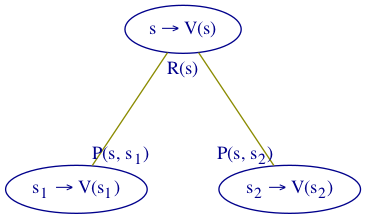
\includegraphics[width=12cm, height=8cm]{mrp_bellman_tree.png}
\end{frame}

\begin{frame}
\frametitle{Key Takeaways from this Chapter}
\pause
\begin{itemize}[<+->]
\item {\bf Markov Property}: Enables us to reason effectively \& compute efficiently in practical systems involving sequential uncertainty
\item {\bf Bellman Equation}: Recursive Expression of the Value Function - this equation (and its MDP version) is the core idea within all Dynamic Programming and Reinforcement Learning algorithms.
\end{itemize}
\end{frame}


\end{document}